\graphicspath{{./figures/capitolo2/}}
\lstset{inputpath = ./programs/capitolo2}
\pgfplotstableset{search path = ./tables/capitolo2}

\chapter{Equazioni alle differenze}

Un'equazione alle differenze lineare di grado $k$ è un'equazione della forma
\begin{equation} \label{eq:equazione-alle-differenze}
\sum_{i=0}^k p_i(n) y_{n+k-i} = g_n,
\quad \text{con $n \geq n_0$, $p_0 \equiv 1$, $p_k(n) \neq 0$}.
\end{equation}
La successione $y_n$ rappresenta l'incognita dell'equazione,
mentre le successioni $p_i(n)$ sono dette \emph{coefficienti}
e la successione $g_n$ \emph{termine noto}.
Se le successioni $p_i(n)$ non dipendono da $n$, allora l'equazione
è detta \emph{a coefficienti costanti}; se il termine noto è nullo,
allora è detta \emph{omogenea}.

La soluzione di un'equazione alle differenze lineare di grado $k$ è
univocamente determinata una volta che sono fissate $k$ condizioni
iniziali $y_{n_0},\dots,y_{n_0+k-1}$.
Questo risultato, che ricorda vagamente quello di esistenza e unicità
per problemi di Cauchy nell'ambito delle equazioni differenziali ordinarie,
è solo il primo di una lunga serie di risultati validi sia per sistemi
dinamici discreti che continui.
Per esempio, anche le equazioni alle differenze lineari omogenee
a coefficienti costanti, proprio come le equazioni differenziali dello
stesso tipo, si possono risolvere associando a un'equazione
il proprio polinomio caratteristico
\[
p(z) = \sum_{i=0}^k p_i \;\! z^{k-i}.
\]
Se le radici $z_1,\dots,z_k$ di tale polinomio sono tutte semplici,
allora la soluzione generica dell'equazione alle differenze ha la forma
\begin{equation} \label{eq:soluzione-radici-distinte}
y_n = c_1 z_1^{n-n_0} + \dots + c_k z_k^{n-n_0},
\end{equation}
che nella sostanza è la stessa che si ottiene nel caso continuo,
con l'unico accorgimento di sostituire le funzioni esponenziali
(autovettori di~$\smash{\frac{d}{dx}}$)
con delle progressioni geometriche (autovettori di~$\Delta$).
Dopodiché, i coefficienti $c_1,\dots,c_k$ possono essere determinati
risolvendo il sistema lineare
\[
\begin{pmatrix*}[c]
1         & \dots & 1         \\
z_1       & \dots & z_k       \\
\vdots    &       & \vdots    \\
z_1^{k-1} & \dots & z_k^{k-1}
\end{pmatrix*}
\begin{pmatrix} c_1 \\ c_2 \\ \vdots \\ c_k \end{pmatrix}
= \begin{pmatrix} y_{n_0} \\ y_{n_0+1} \\ \vdots \\ y_{n_0+k-1} \end{pmatrix}
\]
che si ottiene andando a imporre le condizioni iniziali del problema.
Si può dimostrare che tale matrice, detta \emph{di Vandermonde},
è invertibile perché tutte le radici $z_1,\dots,z_k$ sono per ipotesi distinte.
Nel caso in cui il polinomio caratteristico abbia invece almeno una radice multipla,
la formula \eqref{eq:soluzione-radici-distinte} si generalizza nel modo seguente.
Siano $z_1,\dots,z_\nu$ le radici distinte di $p(z)$,
ciascuna di molteplicità $m_1,\dots,m_\nu$.
Allora la soluzione generica dell'equazione alle differenze ha la forma
\begin{equation} \label{eq:soluzione-radici-multiple}
y_n = \sum_{i=1}^\nu \sum_{j=0}^{m_i-1} c_{ij} (n-n_0)^j z_i^{n-n_0}.
\end{equation}
Anche in questo caso i coefficienti $c_{ij}$ possono essere ricavati
andando a imporre le condizioni iniziali del problema,
e anche in questo caso si può dimostrare che il sistema lineare
associato ammette soluzione unica.
Infine, nel caso di equazioni alle differenze lineari a coefficienti costanti
\emph{non} omogenee, supponendo di conoscere almeno una soluzione
particolare $\bar{y}_n$, si può esprimere l'intero spazio delle soluzioni come
\begin{equation} \label{eq:soluzione-radici-multiple-non-omo}
y_n = \bar{y}_n + \sum_{i=1}^\nu \sum_{j=0}^{m_i-1} c_{ij} (n-n_0)^j z_i^{n-n_0}.
\end{equation}
I numeri complessi $z_1,\dots,z_\nu$ che compaiono in questa formula
sono le radici distinte del polinomio caratteristico dell'equazione omogenea
associata a quella non omogenea di partenza (basta trascurare $g_n$).
Ancora una volta, i coefficienti $c_{ij}$ possono essere ricavati
in modo univoco a partire dalle condizioni iniziali tramite
la soluzione di un sistema lineare.

In questo capitolo applicheremo la teoria delle equazioni
alle differenze al calcolo di importanti quantità matematiche
(come i numeri di Fibonacci), all'analisi della velocità di convergenza
di metodi numerici iterativi (come il metodo delle secanti)
e alla formulazione di alcuni modelli economici a tempo discreto
(dinamica del prezzo di mercato di un bene
e del prodotto interno lordo di una nazione).
Vedremo inoltre come sia possibile determinare le proprietà di stabilità
di una soluzione $y_n$ mediante due criteri costruttivi dovuti a Schur.

\section{Ricorrenza di Fibonacci e instabilità numerica} \label{sec:bitfatale}

La successione dei \emph{numeri di Fibonacci} è definita per ricorrenza come
\[
\left\{
\begin{aligned}
F_n &= F_{n-1} + F_{n-2} \quad \text{per ogni $n \in \N$, $n \geq 2$} \\
F_0 &= 0, \; F_1 = 1
\end{aligned}
\right.
\]
Grazie alla teoria sulle equazioni alle differenze che abbiamo brevemente
esposto all'inizio del capitolo, possiamo scrivere $F_n$ in forma chiusa:
\begin{gather*}
p(z) = z^2-z-1
\qquad z_1 = \frac{1+\sqrt{5}}{2} \eqd \varphi
\qquad z_2 = \frac{1-\sqrt{5}}{2} \eqd \overline{\varphi} \\
%
F_n = c_1 \varphi^n + c_2 \overline{\varphi}^n
\, \text{ con $c_1,c_2$ tali che }
\begin{pmatrix}
1 & 1 \\ 
\varphi & \overline{\varphi}
\end{pmatrix}
\begin{pmatrix} c_1 \\ c_2 \end{pmatrix}
= \begin{pmatrix} 0 \\ 1 \end{pmatrix} \\
%
c_1 = \frac{1}{\sqrt{5}}
\qquad c_2 = -\frac{1}{\sqrt{5}}
\qquad F_n = \frac{1}{\sqrt{5}} (\varphi^n - \overline{\varphi}^n).
\end{gather*}
Ci sarebbe molto da dire sulla storia di questa successione
e sul fascino che essa ha esercitato su generazioni di matematici (e non solo)
nel corso dei secoli, tuttavia non ci sembra il caso di approfondire qui
la questione.
%La successione dei numeri di Fibonacci ha una grande importanza nella
%storia, nella pedagogia e nell'estetica della matematica.
Piuttosto, in questo paragrafo andremo a considerare una versione modificata
della successione di Fibonacci per illustrare con un esempio
le difficoltà che si possono presentare durante il calcolo numerico
della soluzione $y_n$ di un'equazione alle differenze.
Non sempre, infatti, l'algoritmo \emph{ovvio}, cioè quello
riassunto nel Programma \ref{prog:bitfatale}, risulta stabile.
%
\lstinputlisting[float=bp, caption={Soluzione dell'equazione
\eqref{eq:equazione-alle-differenze} tramite sostituzioni in avanti.},
label=prog:bitfatale]{sostituzione_in_avanti.m}
%
Per averne un esempio, si consideri il seguente problema:
\begin{equation} \label{eq:fibonacci-modificata}
\left\{
\begin{aligned}
y_n &= y_{n-1} + y_{n-2} \quad \text{per ogni $n \in \N$, $n \geq 2$} \\
y_0 &= 1, \; y_1 = \overline{\varphi}
\end{aligned}
\right.
\end{equation}
A parte i valori iniziali, la ricorrenza è la stessa
dei numeri di Fibonacci. Dunque
\[
y_n = c_1 \varphi^n + c_2 \overline{\varphi}^n
\, \text{ con $c_1,c_2$ tali che }
\begin{pmatrix}
1 & 1 \\
\varphi & \overline{\varphi}
\end{pmatrix}
\begin{pmatrix} c_1 \\ c_2 \end{pmatrix}
= \begin{pmatrix} 1 \\ \overline{\varphi} \end{pmatrix},
\]
da cui segue che $c_1 = 0$, $c_2 = 1$ e $y_n = \overline{\varphi}^n$.
Dato che $\abs{\overline{\varphi}} < 1$, si ha $y_n \to 0$ per $n \to \infty$.
Tuttavia, andando a calcolare in aritmetica inesatta la successione
\eqref{eq:fibonacci-modificata} si ottiene un andamento qualitativo
sostanzialmente diverso, riportato nella Figura \ref{fig:bitfatale}:
il valore assoluto di $y_n$, che inizialmente decresce come
$\abs{\overline{\varphi}}^n$ (com'è giusto che sia),
a un certo punto ($n = 38$) inizia a crescere come $\varphi^n$.
Cerchiamo di fare luce su questo fenomeno sorprendente.

\begin{figure}[tp]
\centering
\begin{tikzpicture}[trim axis left]
\begin{semilogyaxis}[
	xlabel={$n$},
	ymin = 1e-11, ymax = 10,
	ytickten={-10,-8,...,0},
	width=0.8\textwidth,
	height=0.3\textheight,
	legend style={anchor=south west,at={(0.04,0.04)}}
]
\addplot[only marks, mark=triangle, mark size=2.5pt] table {bitfatale.dat};
\addplot[dashed, domain=0:49] expression {((sqrt(5)-1)/2)^x};
\addplot[densely dashdotted, domain=28:77] expression {1e-16 * ((sqrt(5)+1)/2)^x};
\legend{$\abs{y_n}$, $\abs{\overline{\varphi}}^n$, $\; 10^{-16} \varphi^n$}
\end{semilogyaxis}
\end{tikzpicture}
\caption{Calcolo della successione \eqref{eq:fibonacci-modificata}
in aritmetica inesatta}
\label{fig:bitfatale}
\end{figure}

Iniziamo osservando che la costante $\overline{\varphi}$ non è un numero
di macchina, quindi quando approssimiamo il vettore delle condizioni iniziali
$(1, \overline{\varphi})$ con $(1, r(\overline{\varphi}))$ andiamo a commettere
un errore relativo (in norma) dell'ordine di $\varepsilon$, epsilon di macchina.
Anche se d'ora in poi non ci fossero altri errori dovuti all'aritmetica finita,
l'algoritmo \ref{prog:bitfatale} andrebbe a risolvere in modo esatto il problema
perturbato
\begin{equation*} \label{eq:fibonacci-perturbata}
\left\{
\begin{aligned}
y_n &= y_{n-1} + y_{n-2} \quad \text{per ogni $n \in \N$, $n \geq 2$} \\
y_0 &= 1, \; y_1 = r(\overline{\varphi})
\end{aligned}
\right.
\end{equation*}
che ha chiaramente soluzione diversa dal problema originale
\eqref{eq:fibonacci-modificata}.
Indichiamo con $y_n'$ questa nuova soluzione e siano $c_1',c_2'$
le costanti tali che $y_n' = c_1' \varphi^n + c_2' \overline{\varphi}^n$.
Dato che il vettore $(c_1',c_2')$ si ottiene dalla soluzione di un sistema
lineare con termine noto $(1, r(\overline{\varphi}))$,
e dato che la distanza relativa tra $(1, \overline{\varphi})$
e $(1, r(\overline{\varphi}))$ è dell'ordine di $\varepsilon$,
allora anche la distanza relativa tra $(c_1,c_2)$
e $(c_1',c_2')$ sarà dell'ordine di $\varepsilon$.
In particolare, si avrà $\abs{c_1'} = \abs{c_1'-c_1} \approx \varepsilon$.
Dunque, dato che $c_1'$ non è nullo, è chiaro perché
a un certo punto il termine $c_1' \varphi^n$
prenda il sopravvento sul termine $c_2' \overline{\varphi}^n$.
La stima $c_1' \approx \varepsilon$, $c_2' \approx 1$ ci permette anche
di calcolare il valore di $n$ per cui avviene il sorpasso:
\[
c_1' \varphi^n = c_2' \abs{\overline{\varphi}}^n
\quad \varepsilon \varphi^n \approx \abs{\overline{\varphi}}^n
\quad \log(\varepsilon) + n \log(\varphi) \approx n \log(\abs{\overline{\varphi}})
\quad n \approx \frac{-\log(\varepsilon)}
                     {\log(\varphi) - \log(\abs{\overline{\varphi}})}
        \approx 38
\]
Questo valore di $n$ è in perfetto accordo con i dati sperimentali
riportati in Figura \ref{fig:bitfatale}, a conferma del fatto che
il fenomeno di instabilità numerica è stato analizzato correttamente.

Ora, rimane da stabilire se sia possibile trovare un'alternativa stabile
all'algoritmo \ref{prog:bitfatale} per la soluzione del problema
\ref{eq:fibonacci-modificata}. La risposta è \emph{no}, perché si può dimostrare
(basta rendere rigorosa l'analisi già svolta) che il problema del calcolo
di $y_n$ dati $y_0 = 1$ e $y_1 = \overline{\varphi}$ ha numero di
condizionamento relativo%
\footnote{Stiamo quindi analizzando il condizionamento relativo nel caso pessimo.
Ma il numero di condizionamento assoluto cresce come $\varphi^n$ in ogni caso,
cioè a prescindere dai valori di $y_0$ e $y_1$.}
che cresce come $\varphi^n$.
Più in generale, si può dimostrare che il calcolo della soluzione di un'equazione
alle differenze a coefficienti costanti è sempre mal condizionato se
almeno una delle radici del polinomio caratteristico ha modulo
maggiore di 1, come in questo caso.
Vista l'importanza del concetto di stabilità, torneremo a parlarne
nel Paragrafo \ref{sec:schur}.
Prima, però, vediamo un'applicazione della formula chiusa
per la ricorrenza di Fibonacci al calcolo della velocità di convergenza
del metodo delle secanti.

\section{Metodo delle secanti} \label{sec:secanti}

Il metodo delle secanti è un metodo numerico iterativo per la ricerca
di zeri di funzioni scalari $f \colon \R \supseteq \Omega \to \R$.
Scelti due punti di partenza distinti $x_0$ e $x_1$
in $\Omega$, il metodo consiste nell'iterazione della formula
\begin{equation} \label{eq:definizione-secanti}
x_{n+1} = x_n - f(x_n) \frac{x_n-x_{n-1}}{f(x_n)-f(x_{n-1})}.
\end{equation}
Il nome \emph{metodo delle secanti} deriva dall'interpretazione
geometrica che si può associare a questa formula.
Osserviamo che il metodo è ben definito solo se a ogni passo
i valori di $f$ in $x_n$ e $x_{n-1}$ sono distinti.
Nel caso in cui ricorrano le giuste condizioni sia sulla funzione $f$,
sia sui valori di innesco $x_0$ e $x_1$, la
successione delle iterate $\{x_n\}$ converge a un
$x \in \Omega$ tale che $f(x) = 0$.

Il metodo delle secanti condivide con il più noto metodo di Newton
gran parte dei pregi e dei difetti: entrambi i metodi, infatti,
possiedono convergenza superlineare per funzioni $C^2$ nei pressi
di radici semplici (più lenta per radici multiple, come vedremo in seguito),
ma la convergenza è assicurata solo se la stima iniziale si trova
in un intorno opportuno della soluzione, detto \emph{bacino di attrazione} del metodo,
di cui spesso non si hanno informazioni a priori.
Per questo si parla, per entrambi i metodi, di convergenza \emph{locale},
anziché \emph{globale}.

Rispetto al metodo di Newton, il metodo delle secanti ha il vantaggio
di non richiedere né la conoscenza né il calcolo della derivata della funzione.
Inoltre, anche rispetto al metodo di Newton alle differenze,
il metodo delle secanti richiede una sola valutazione di funzione
per ogni iterazione, anziché due.
Per quanto riguarda gli svantaggi, non è immediato generalizzare
il metodo delle secanti a sistemi di $m$ equazioni in $m$ incognite;
lo si può comunque fare con il \emph{metodo di Broyden},
ma quest'ultimo è decisamente più complesso da comprendere
e da implementare rispetto al metodo di Newton.
Inoltre, l'ordine di convergenza del metodo delle secanti non è quadratico,
come nel caso del metodo di Newton, bensì pari alla sezione aurea
(circa 1.618) e quindi inferiore.
Le proprietà esatte di convergenza del metodo delle secanti sono riassunte
nel seguente teorema:

\begin{teor} \label{teor:convergenza-superlineare-secanti}
Sia $\Omega$ un aperto di $\R$ e $f \colon \Omega \to \R$ una funzione $C^2(\Omega)$.
Sia $x \in \Omega$ una radice semplice di $f$,
ossia un valore per cui $f(x) = 0$, ma $f'(x) \neq 0$.
Siano
\[
\varphi = \frac{1+\sqrt{5}}{2},
\quad \overline{\varphi} = \frac{1-\sqrt{5}}{2},
\quad M = \frac{\abs{f''(x)}}{2\abs{f'(x)}},
\quad e_n = x - x_n.
\]
Supponiamo che il metodo delle secanti non
abbia terminazione finita, cioè $e_n \neq 0$ per ogni $n \in \N$.
Allora esiste $U \subseteq \Omega$ intorno di $x$ tale che,
per ogni scelta di $x_0$ e $x_1$ distinti in $U$, si ha che
\begin{enumerate}
\item La successione $\{x_n\}_{n\in\N}$ è ben definita
	e inclusa in $U$.
\item La successione $\{x_n\}_{n\in\N}$ converge a $x$.
\item Se $f''(x) \neq 0$, la convergenza è superlineare, con ordine $\varphi$:
	\[ \lim_{n \to \infty} \frac{\abs{e_{n+1}}}{\abs{e_n}^\varphi}
	= M^{\varphi-1}. \]
\end{enumerate}
\end{teor}

\begin{proof}
Per il teorema di Lagrange e la continuità di $f'$, esiste un intorno $U$ per cui
\begin{equation} \label{eq:disuguaglianza-rapporto-errori}
\begin{split}
\abs{\frac{e_{n+1}}{e_n}}
&= \abs{\frac{x-x_{n+1}}{x-x_n}}
 = \abs{\frac{1}{x-x_n}
	   \left(x - x_n + f(x_n) \frac{x_n-x_{n-1}}{f(x_n)-f(x_{n-1})}\right)} \\
&= \abs{1 - \frac{f(x)-f(x_n)}{x-x_n} \frac{x_n - x_{n-1}}{f(x_n)-f(x_{n-1})}}
= \abs{1 - \frac{f'(\xi)}{f'(\zeta)}}
< \frac{1}{2}.
\end{split}
\end{equation}
A questo punto, per induzione, si deduce che
\[
\abs{e_n} < \frac{1}{2^{n-1}} \abs{e_1}.
\]
Questa disuguaglianza dimostra i primi due punti dell'enunciato.
Per quanto riguarda il terzo punto, riprendiamo la catena di uguaglianze
precedente e sfruttiamo la regolarità $C^2$ di $f$:
\begin{gather*}
\frac{\abs{e_{n+1}}}{\abs{e_n} \abs{e_{n-1}}}
= \frac{1}{\abs{e_{n-1}}} \abs{1-\frac{f[x_n,x]}{f[x_{n-1},x_n]}}
= \frac{1}{\abs{x-x_{n-1}}} \abs{\frac{f[x_{n-1},x_n]-f[x_n,x]}{f[x_{n-1},x_n]}}
= \frac{\abs{f[x_{n-1},x_n,x]}}{\abs{f[x_n,x_{n-1}]}} \\
\lim_{n \to \infty} \frac{\abs{e_{n+1}}}{\abs{e_n} \abs{e_{n-1}}}
= \lim_{n \to \infty} \frac{\abs{f[x_{n-1},x_n,x]}}{\abs{f[x_n,x_{n-1}]}}
= \lim_{n \to \infty} \frac{\abs{f''(\eta_n)}}{2\abs{f'(\zeta_n)}}
= \frac{\abs{f''(x)}}{2\abs{f'(x)}}
= M.
\end{gather*}
Per alleggerire i calcoli, abbiamo fatto uso delle \emph{differenze divise}
e del relativo teorema del valor medio.
Il risultato ottenuto ci dice che, per valori di $n$ grandi,
\begin{equation} \label{eq:approssimazione-secanti}
\abs{e_{n+1}} \approx M \abs{e_n} \abs{e_{n-1}}.
\end{equation}
Supponiamo per il momento che tale approssimazione sia esatta.
Allora, moltiplicando entrambi i membri per $M \neq 0$ e passando ai logaritmi,
si avrebbe
\[
\log(M\abs{e_{n+1}}) = \log(M\abs{e_n}) + \log(M\abs{e_{n-1}})
\]
Se ora definiamo $y_n = \log(M\abs{e_n})$, possiamo riconoscere
ancora una volta la ricorrenza di Fibonacci,
di cui conosciamo la formula chiusa per il termine $n$-esimo:
\[
y_n = c_1 \varphi^n + c_2 \overline{\varphi}^n.
\]
Allora possiamo concludere che
\begin{equation} \label{eq:limite-tesi-secanti}
\begin{aligned}
\lim_{n \to \infty} \frac{\abs{e_{n+1}}}{\abs{e_n}^\varphi}
&= \lim_{n \to \infty} \frac{ M^{-1}       \exp(y_{n+1}) }
                           { M^{-\varphi} \exp(y_n \varphi) }
 = \lim_{n \to \infty} M^{\varphi-1} \exp(y_{n+1}-y_n \varphi) \\
&= \lim_{n \to \infty} M^{\varphi-1}
	\exp(c_1 \varphi^{n+1} + c_2 \overline{\varphi}^{n+1} -
	     c_1 \varphi^{n+1} - c_2 \overline{\varphi}^n \varphi) \\
&= \lim_{n \to \infty} M^{\varphi-1}
	\exp(c_2 \overline{\varphi}^{n+1} - c_2 \overline{\varphi}^n \varphi)
 = M^{\varphi-1}.
\end{aligned}
\end{equation}

La dimostrazione che abbiamo dato, per poter essere del tutto rigorosa,
richiede un'analisi più approfondita dell'approssimazione
\eqref{eq:approssimazione-secanti}.
Si può dimostrare che esiste $k > 0$ tale che
\begin{equation} \label{eq:stima-asintotica-secanti}
M - k 2^{-n}
\leq \frac{\abs{e_{n+1}}}{\abs{e_n} \abs{e_{n-1}}}
\leq M + k 2^{-n}.
\end{equation}
A questo punto si ottengono due disequazioni
\[
\left\{
\begin{aligned}
& (M - k 2^{-n}) \abs{e_{n-1}} (M - k 2^{-n}) \abs{e_n}
	\leq (M - k 2^{-n}) \abs{e_{n+1}} \\
& (M + k 2^{-n}) \abs{e_{n-1}} (M + k 2^{-n}) \abs{e_n}
	\geq (M + k 2^{-n}) \abs{e_{n+1}}
\end{aligned}
\right.
\]
e come prima possiamo passare ai logaritmi per ottenere in entrambi
i casi la ricorrenza di Fibonacci, anche se con valori iniziali differenti
(e dipendenti da $n$). Tramite un opportuno teorema del confronto
possiamo stabilire che
\[
\left\{
\begin{aligned}
& \log((M - k 2^{-n}) \abs{e_n}) \geq c_1(n) \varphi^n + c_2(n) \overline{\varphi}^n \\
& \log((M + k 2^{-n}) \abs{e_n}) \leq d_1(n) \varphi^n + d_2(n) \overline{\varphi}^n
\end{aligned}
\right.
\]
e questo è sufficiente per dimostrare la tesi con
lo stesso approccio della \eqref{eq:limite-tesi-secanti}.
Stavolta i termini $c_1(n) \varphi^{n+1}$ e $d_1(n) \varphi^{n+1}$
presenti nell'argomento della funzione esponenziale
non si cancellano, perché $c_1(n) \neq d_1(n)$, ma in compenso
$c_1(n) - d_1(n) = O(2^{-n})$ e quindi
\[
(c_1(n)-d_1(n))\varphi^{n+1} \to 0. \qedhere
\]
\end{proof}

Dedichiamo il resto del paragrafo al confronto tra il risultato teorico
appena ottenuto e le proprietà di convergenza che si osservano in pratica.
A tal fine, si consideri la seguente implementazione del metodo delle secanti:
\vspace{1.5ex}
\lstinputlisting[frame={},caption={Metodo delle secanti},
label=prog:secanti]{secanti.m}
\vspace{1ex}
Molti dettagli del funzionamento del programma sono illustrati tramite
commenti all'interno del codice.
Abbiamo inoltre cercato di attenerci il più possibile alla notazione adottata
finora, specialmente per quanto riguarda la costruzione della tabella
\texttt{T}.
La prima colonna della tabella contiene il numero $n$ dell'iterazione corrente.
La seconda e la terza colonna contengono un'approssimazione in aritmetica inesatta
di $x_n$ e $f(x_n)$.
La quarta colonna contiene la distanza tra $x_n$ e $x_{n-1}$.
La quinta e la sesta colonna contengono i rapporti
\[
R_1 = \frac{\abs{x_n-x_{n-1}}}{\abs{x_{n-1}-x_{n-2}}}
\quad \text{ e } \quad
R_\varphi = \frac{\abs{x_n-x_{n-1}}}{\abs{x_{n-1}-x_{n-2}}^\varphi},
\]
il cui significato verrà chiarito in seguito.
Commentiamo ora brevemente il criterio di arresto utilizzato
(linea di codice 64), comune a tutti i metodi iterativi.
Per valutare la convergenza di un metodo numerico, l'ideale sarebbe
poter monitorare direttamente l'errore $\abs{e_n} = \abs{x-x_n}$,
il che però è ovviamente impossibile perché il valore di $x$ è a priori incognito.
Il seguente teorema offre un'alternativa indiretta:

\begin{teor} \label{teor:indicatore-convergenza}
In ogni metodo numerico iterativo si ha che
\[
1 - \frac{\abs{e_n}}{\abs{e_{n-1}}}
\leq \frac{\abs{x_n-x_{n-1}}}{\abs{e_{n-1}}}
\leq 1 + \frac{\abs{e_n}}{\abs{e_{n-1}}}
\]
\end{teor}

\begin{proof}
Segue da un'applicazione opportuna della disuguaglianza triangolare.
\end{proof}

\noindent Pertanto, se vale la disuguaglianza
\eqref{eq:disuguaglianza-rapporto-errori}, come nella dimostrazione del
Teorema~\ref{teor:convergenza-superlineare-secanti},
si vede facilmente che
\[
\frac{1}{2} \leq \frac{\abs{x_n-x_{n-1}}}{\abs{e_{n-1}}} \leq \frac{3}{2},
\]
cioè che la distanza tra due iterazioni consecutive $x_n$ e $x_{n-1}$
è una buona approssimazione dell'errore all'iterazione $n-1$.
Addirittura, se valgono tutte le ipotesi dello stesso teorema, si ha che
la convergenza è superlineare e quindi
\begin{equation} \label{eq:approssimazione-errore}
\lim_{n \to \infty} \frac{\abs{e_n}}{\abs{e_{n-1}}} = 0
\quad \text{implica che} \quad
\lim_{n \to \infty} \frac{\abs{x_n-x_{n-1}}}{\abs{e_{n-1}}} = 1,
\end{equation}
cioè l'approssimazione diventa ancora migliore per $n$ sufficientemente grande.
Le distanze $\abs{x_n-x_{n-1}}$ nella quarta colonna della tabella \texttt{T}
possono quindi essere interpretate come delle stime dell'errore $\abs{e_{n-1}}$,
a patto che i valori $x_{n-1}$ e $x_{n-2}$ siano contenuti
nell'intorno $U$ di $x$ a cui si fa riferimento nella disequazione
\eqref{eq:disuguaglianza-rapporto-errori}.
I criteri di arresto \emph{esatti} sugli errori assoluti e relativi
\[
\abs{e_n} \leq t_a
\qquad \frac{\abs{e_n}}{\abs{x}} \leq t_r
\]
possono così essere sostituiti in modo altrettanto efficace dai controlli numerici
\[
\abs{x_{n+1}-x_n} \leq t_a
\qquad \frac{\abs{x_{n+1}-x_n}}{\abs{x_{n+1}}} \leq t_r,
\]
spesso uniti in un unico \emph{criterio di arresto misto sulle iterate}
\[
\abs{x_{n+1}-x_n} \leq t_a + t_r \abs{x_{n+1}}.
\]
Tra i due criteri di arresto (assoluto e relativo), quello di gran lunga
più utile è quello relativo, perché garantisce un certo numero
di cifre significative corrette nel risultato (una richiesta naturale,
lavorando con numeri a virgola mobile anziché fissa) e perché permette
facilmente di capire quanto la precisione richiesta sul risultato
sia vicina alla precisione massima ottenibile con i numeri di macchina
(basta confrontare $t_r$ con $\varepsilon$).
Tuttavia, il criterio misto risulta in generale preferibile
a uno puramente relativo, perché in grado di gestire correttamente
anche il caso $x \approx 0$, in cui gli errori relativi perdono
di significato.

Cambiando punto di vista, un'altra possibilità per il criterio di arresto
sarebbe quella di monitorare la grandezza $\abs{f(x_n)}$.
Dato che stiamo cercando uno zero della funzione $f$, sembra naturale
fermarsi una volta che
\begin{equation} \label{eq:controllo-sulla-funzione}
\abs{f(x_n)} \leq t_f.
\end{equation}
Se $x$ è una radice semplice, allora dalla formula di Taylor
per $f$ con centro $x$ segue l'approssimazione
\[
\abs{f(x_n)} \approx \abs{f'(x)} \abs{x-x_n} = \abs{f'(x)} \abs{e_n}
\]
e quindi il controllo \eqref{eq:controllo-sulla-funzione} è sostanzialmente
equivalente al criterio di arresto sull'errore assoluto con tolleranza
\[
t_a = \abs{f'(x)}^{-1} t_f,
\]
a patto che il metodo numerico stia convergendo a $x$.
Se invece $x$ è una radice multipla, il controllo \eqref{eq:controllo-sulla-funzione}
è genuinamente diverso da quelli visti in precedenza, anche se continua
a sussistere una certa relazione in base alla formula di Taylor.

Chiariamo ora il significato dei rapporti $R_1$ e $R_\varphi$.
Così come le distanze $\abs{x_n-x_{n-1}}$ possono essere interpretate
come stime degli errori assoluti $\abs{e_{n-1}}$, i rapporti tra le distanze
\[
\frac{\abs{x_n-x_{n-1}}}{\abs{x_{n-1}-x_{n-2}}}
\quad \text{e} \quad
\frac{\abs{x_n-x_{n-1}}}{\abs{x_{n-1}-x_{n-2}}^\varphi}
\]
misurati durante le prime \code{nmax} iterazioni possono essere monitorati per
avere una stima dell'andamento asintotico dei rapporti tra gli errori
\[
\frac{\abs{e_{n-1}}}{\abs{e_{n-2}}}
\quad \text{e} \quad
\frac{\abs{e_{n-1}}}{\abs{e_{n-2}}^\varphi},
\]
dai quali dipende l'ordine di convergenza del metodo numerico.
Naturalmente ci sono due problemi con questo approccio.
Il primo riguarda la possibilità di approssimare $\abs{e_{n-1}}$
con $\abs{x_n-x_{n-1}}$ sotto segno di limite, senza però sapere a priori
che il metodo stia convergendo con una certa velocità (proprio
perché vorremmo dedurre l'ordine di convergenza del metodo a partire
dagli indicatori $R_1$ e $R_\varphi$, e non viceversa).
Il secondo problema riguarda l'analisi di un numero finito di termini:
anche ammesso che i limiti dei rapporti esistano finiti e che
\[
\lim_{n \to \infty} \frac{\abs{x_n-x_{n-1}}}{\abs{x_{n-1}-x_{n-2}}}
= \lim_{n \to \infty} \frac{\abs{e_{n-1}}}{\abs{e_{n-2}}}
\quad \text{e} \quad
\lim_{n \to \infty} \frac{\abs{x_n-x_{n-1}}}{\abs{x_{n-1}-x_{n-2}}^\varphi}
= \lim_{n \to \infty} \frac{\abs{e_{n-1}}}{\abs{e_{n-2}}^\varphi},
\]
non è affatto detto che i primi \texttt{nmax} termini delle successioni
$R_1$ o $R_\varphi$ siano in qualche modo rappresentativi del
valore del limite delle successioni stesse.
L'analisi degli indicatori $R_1$ e $R_\varphi$ non è quindi sostitutiva di
uno studio rigoroso dell'ordine di convergenza del metodo numerico,
anche se quest'ultimo può essere estremamente complesso
in molti casi di interesse pratico (al punto da essere talvolta un problema aperto).
In analisi numerica capita in effetti che ci si debba
accontentare di un'evidenza empirica riguardo all'ordine di convergenza
di un metodo, piuttosto che di una certezza matematica a riguardo.

Tornando al metodo delle secanti e al Programma \ref{prog:secanti},
se valgono le ipotesi del Teorema \ref{teor:convergenza-superlineare-secanti},
e quindi la convergenza è superlineare, ci aspettiamo che l'indicatore $R_1$
nella quinta colonna della tabella \texttt{T} tenda a zero, e che allo stesso
tempo l'indicatore $R_\varphi$ nella sesta colonna tenda a $M^{\varphi-1}$.
In effetti in seguito avremo modo di osservare tali andamenti,
a conferma del fatto che teoria e pratica si sostengono a vicenda.
In tutto l'elaborato cercheremo sempre questa concordanza, perché ci darà
la ragionevole certezza di aver interpretato bene i risultati teorici,
e allo stesso tempo di aver implementato correttamente i metodi numerici.

A conclusione di questo paragrafo, commentiamo i risultati dell'esecuzione
del Programma~\ref{prog:secanti} con alcuni esempi che ci sono sembrati significativi.

\begin{esem}
Consideriamo la funzione polinomiale $f(x) = x^2-x-1$,
le cui due radici semplici sono proprio $\varphi$ e $\bar{\varphi}$.
Nella Tabella \ref{tab:esempio-secanti-1} sono riportati i risultati dell'esecuzione
del metodo delle secanti con valori iniziali $x_0 = 3$ e $x_1 = 2$,
e criterio di arresto misto sulle iterate con $t_a = t_r = 10^{-12}$.
Possiamo osservare che i valori iniziali si trovano all'interno
del bacino di attrazione $U$ di $\varphi$, quindi sono verificate
le ipotesi del Teorema \ref{teor:convergenza-superlineare-secanti}
e sappiamo che la convergenza a tale radice sarà superlineare.
In effetti, l'indicatore $R_1$ tende a zero, mentre l'indicatore
$R_\varphi$ tende a
\[
M^{\varphi-1}
= \left( \frac{2}{2(2\varphi-1)} \right)^{\varphi-1}
= (2\varphi-1)^{1-\varphi}
\approx 0.608.
\]
\end{esem}

\begin{esem}
Consideriamo la funzione $f(x) = x^{-1} - 10^{-6}$, la cui unica radice è $10^6$.
Supponiamo di ignorare l'ordine di grandezza di tale radice,
e di scegliere quindi dei valori di innesco piuttosto lontani da essa,
ad esempio $x_0 = 1$ e $x_1 = 2$.
Nella Tabella \ref{tab:esempio-secanti-2} sono riportati i risultati dell'esecuzione
del metodo delle secanti con criterio di arresto misto sulle iterate
con $t_a = t_r = 10^{-12}$.
Possiamo osservare che per le prime 30 iterazioni il metodo sembra divergere:
il valore di $R_1$ è maggiore di $1$, e sia $x_n$ che $\abs{x_n-x_{n-1}}$
crescono in modo apparentemente illimitato.
Tuttavia, a partire dall'iterazione numero 30,
quando $x_n$ è finalmente nei pressi della radice,
il metodo inizia improvvisamente a convergere,
e come previsto dalla teoria lo fa in modo superlineare,
dato che la radice è semplice.
\end{esem}

\begin{esem}
Consideriamo invece la funzione $f(x) = x/(x^2+1)$, la cui unica radice è 0.
Si può dimostrare che tale radice ha un bacino di convergenza $U$ limitato
e incluso nell'intervallo $(-1,1)$.
Scegliamo deliberatamente punti iniziali esterni a $U$, per esempio
$x_0 = 1$ e $x_1 = 2$. Nella Tabella \ref{tab:esempio-secanti-3} sono
riportati i risultati dell'esecuzione del metodo delle secanti,
che termina soltanto perché $n$ raggiunge il numero massimo di iterazioni
\code{nmax}, che in questo esempio abbiamo fissato uguale a 20.
Osserviamo che lo storico di convergenza è in tutto e per tutto
simile a quello dell'esempio precedente, con l'unica differenza che
in questo caso sappiamo che il metodo delle secanti non convergerà mai.
A che conclusione saremmo quindi giunti nell'esempio precedente
se avessimo ignorato l'esistenza di una radice in $x = 10^6$
e ci fossimo fermati dopo sole 20 iterazioni?
Questo esempio ci fa riflettere ancora una volta sulla
differenza tra evidenza empirica e certezza matematica.
Osserviamo anche un'altra cosa. Nonostante il metodo diverga,
i valori di $f(x_n)$ tendono lo stesso a zero.
Così, potrebbe risultare impropriamente soddisfatto il criterio
di arresto basato sui valori della funzione.
Per questo è importante scegliere $t_f = 0$ in questo esempio.
\end{esem}

\begin{esem}
Consideriamo la funzione strettamente crescente $f(x) = x^3 + \sqrt[5]{x}$,
la cui unica radice è 0.
Anche se tale funzione non ha regolarità $C^2$, requisito necessario
per l'applicazione del Teorema \ref{teor:convergenza-superlineare-secanti},
non possiamo escludere a priori che il metodo delle secanti converga lo stesso.
Scegliamo come valori iniziali $x_0 = 10$ e $x_1 = 9$.
I risultati dell'esecuzione del metodo delle secanti
sono riportati nella Tabella \ref{tab:esempio-secanti-4}.
In effetti, durante le prime 10 iterazioni il metodo sembra convergere a zero,
ma poi a partire dalle iterazioni successive diventa evidente che il metodo
sta incontrando qualche ostacolo (il flesso a tangente verticale
nei pressi dello 0) che gli impedisce di continuare a convergere.
Il metodo raggiunge così uno stallo sotto forma di ciclo di periodo
quattro.
In questo esempio, si può dimostrare che la radice $x = 0$ ha un bacino di
convergenza $U$ vuoto. Anche in questo caso, dunque, il metodo delle secanti
termina soltanto perché $n$ raggiunge il numero massimo di iterazioni
\code{nmax}, che abbiamo fissato uguale a 28.
\end{esem}

Questi primi quattro esempi mostrano chiaramente che la convergenza
di un metodo iterativo (nello specifico, del metodo delle secanti)
non può essere stabilita in modo puramente empirico.
Vediamo ora altri due esempi: uno relativo a radici doppie,
e uno relativo a radici semplici in cui la derivata seconda è nulla.

\begin{esem}
Consideriamo la funzione $f(x) = x^2$, la cui unica radice è ovviamente
0, ed è una radice doppia. Anche in questo caso non è quindi possibile
applicare il Teorema \ref{teor:convergenza-superlineare-secanti}.
Nella Tabella \ref{tab:esempio-secanti-5} sono riportati i risultati
dell'esecuzione del metodo delle secanti con valori iniziali
$x_0 = 1$ e $x_1 = 0.9$, e criterio di arresto assoluto con $t_a = 10^{-6}$.
Osserviamo che il metodo risulta convergente, ma con ordine apparentemente
minore di $\varphi$: l'indicatore $R_\varphi$ sembra infatti tendere a~$+\infty$.
Al contrario, l'indicatore $R_1$ sembra convergere a una quantità positiva
strettamente minore di 1 (apparentemente, $\varphi-1$),
il che ci porta a concludere che il metodo delle
secanti stia convergendo con velocità lineare.
\end{esem}

\begin{esem}
Consideriamo la funzione $f(x) = e^x - 1 - x^2/2$, la cui unica radice è 0,
ed è una radice singola. Purtroppo, dato che per costruzione $f''(0) = 0$,
non possiamo applicare il terzo punto del
Teorema \ref{teor:convergenza-superlineare-secanti}, che garantisce
velocità di convergenza superlineare. In realtà, la velocità di convergenza
osservata è addirittura maggiore: nella Tabella \ref{tab:esempio-secanti-6}
sono riportati i risultati dell'esecuzione con valori iniziali
$x_0 = 1$ e $x_1 = 0.9$, e criterio di arresto misto con
$t_a = t_r = 10^{-12}$.
Leggendo la tabella, si osserva che l'indicatore $R_\varphi$ tende a zero,
segno che l'ordine di convergenza è maggiore di $	\varphi$.
\end{esem}

\pgfplotstableset{
	columns/n/.style={column type=r, int detect, column name=$n$},
	columns/xn/.style={sci sep align=c, sci precision = 14, column name=$x_n$},
	columns/fxn/.style={sci sep align=c, column name=$f(x_n)$},
	columns/absdx/.style={sci sep align=c, column name=$\scriptstyle{\abs{x_n-x_{n-1}}}$},
	columns/dxratio/.style={sci sep align=c, column name=$R_1$},
	columns/dxratiophi/.style={sci sep align=c, column name=$R_\varphi$}
}

\begin{table}[p]
\caption{Esecuzione del Programma \ref{prog:secanti} con $f(x) = x^2-x-1$}
\label{tab:esempio-secanti-1}
\centering
\begin{small}
\pgfplotstabletypeset{secanti1.dat}
\end{small}
\end{table}

\begin{table}[bp]
\caption{Esecuzione del Programma \ref{prog:secanti} con $f(x) = 1/x - 10^{-6}$}
\label{tab:esempio-secanti-2}
\centering
\begin{small}
\pgfplotstabletypeset{secanti2.dat}
\end{small}
\end{table}

\begin{table}[p]
\caption{Esecuzione del Programma \ref{prog:secanti} con $f(x) = x/(x^2+1)$}
\label{tab:esempio-secanti-3}
\centering
\begin{small}
\pgfplotstabletypeset{secanti3.dat}
\end{small}
\end{table}

\begin{table}[p]
\caption{Esecuzione del Programma \ref{prog:secanti} con $f(x) = x^3 + \sqrt[5]{x}$}
\label{tab:esempio-secanti-4}
\centering
\begin{small}
\pgfplotstabletypeset{secanti4.dat}
\end{small}
\end{table}

\begin{table}[p]
\caption{Esecuzione del Programma \ref{prog:secanti} con $f(x) = x^2$}
\label{tab:esempio-secanti-5}
\centering
\begin{small}
\pgfplotstabletypeset{secanti5.dat}
\end{small}
\end{table}

\begin{table}[p]
\caption{Esecuzione del Programma \ref{prog:secanti} con $f(x) = e^x - 1 - x^2/2$}
\label{tab:esempio-secanti-6}
\centering
\begin{small}
\pgfplotstabletypeset{secanti6.dat}
\end{small}
\end{table}

\section{Stabilità e criteri di Schur} \label{sec:schur}

%Come preannunciato alla fine del paragrafo \ref{sec:bitfatale},
Torniamo ora a occuparci di stabilità.
Alla fine del paragrafo \ref{sec:errore} avevamo dato la definizione
informale di algoritmo \emph{stabile}; diamo ora invece la definizione
di \emph{soluzione stabile} di un'equazione alle differenze.
Per semplicità, limitiamoci al caso di un'equazione lineare
a coefficienti costanti:

\begin{defi}[Stabilità di una soluzione]
Sia $\{\bar{y}_n\}_{n \geq n_0}$ una soluzione dell'equazione alle differenze lineare
\begin{equation} \label{eq:equazione-alle-differenze-lin-cc}
\sum_{i=0}^k p_i y_{n+k-i} = g_n.
\end{equation}
Se per ogni altra soluzione $\{y_n\}_{n \geq n_0}$ si ha che
$\sup_{n \geq n_0} \abs{\bar{y}_n-y_n} < +\infty$, allora
la soluzione $\bar{y}_n$ si dice \emph{stabile}, altrimenti \emph{instabile}.
Se per ogni altra soluzione $\{y_n\}_{n \geq n_0}$ si ha che
$\sup_{n \geq n_0} \abs{\bar{y}_n-y_n} = 0$, allora la soluzione $\bar{y}_n$
si dice \emph{asintoticamente stabile}.
\end{defi}

In realtà, nel caso di un'equazione lineare a coefficienti costanti,
le proprietà di stabilità non dipendono dalla soluzione scelta,
ma solamente dall'equazione stessa.

\begin{teor}[Caratterizzazione delle soluzioni stabili]
\label{teor:sol-stabili-eq-alle-diff-lineare}
Sia $p(z)$ il polinomio caratteristico dell'equazione omogenea
associata alla \eqref{eq:equazione-alle-differenze-lin-cc},
e siano $z_1,\dots,z_\nu$ le radici di $p(z)$, ciascuna di molteplicità
$m_1,\dots,m_\nu$. Allora valgono le seguenti:
\begin{enumerate}
\item Se esiste almeno una soluzione stabile dell'equazione
	\eqref{eq:equazione-alle-differenze-lin-cc}, allora si ha che
	$\abs{z_i} \leq 1$ per ogni $i = 1,\dots,\nu$, e inoltre
	$m_i = 1$ per ogni radice $z_i$ tale che $\abs{z_i} = 1$.
\item Se $\abs{z_i} \leq 1$ per ogni $i = 1,\dots,\nu$, e inoltre
	$m_i = 1$ per ogni radice $z_i$ tale che $\abs{z_i} = 1$, allora
	tutte le soluzioni dell'equazione \eqref{eq:equazione-alle-differenze-lin-cc}
	sono stabili.
\item Se esiste almeno una soluzione asintoticamente stabile dell'equazione
	\eqref{eq:equazione-alle-differenze-lin-cc}, allora si ha che
	$\abs{z_i} < 1$ per ogni $i = 1,\dots,\nu$.
\item Se $\abs{z_i} < 1$ per ogni $i = 1,\dots,\nu$, allora tutte le soluzioni
	dell'equazione \eqref{eq:equazione-alle-differenze-lin-cc}
	sono asintoticamente stabili.
\end{enumerate}
\end{teor}

\begin{proof}
Segue essenzialmente dal fatto che la differenza tra due soluzioni
dell'equazione \eqref{eq:equazione-alle-differenze-lin-cc}
è una soluzione dell'equazione omogenea associata, e pertanto
può essere scritta nella forma \eqref{eq:soluzione-radici-multiple}.
A quel punto si sfrutta il fatto che
\[
\sup_{n \geq n_0} \abs{c_{ij} (n-n_0)^j z_i^{n-n_0}} = 0
\]
se e solo se $\abs{z_i} < 1$, e che
\[
\sup_{n \geq n_0} \abs{c_{ij} (n-n_0)^j z_i^{n-n_0}} < +\infty
\]
se e solo se $\abs{z_i} \leq 1$, a patto che $j = 0$ nel caso in cui $\abs{z_i} = 1$.
\end{proof}

Come corollario, osserviamo che le soluzioni possono quindi essere tutte stabili,
oppure tutte instabili, ma non sono ammesse vie di mezzo. Questo fenomeno
è tipico del caso lineare.

La formula risolutiva \eqref{eq:soluzione-radici-multiple}
è alla base anche di un'altra considerazione importante, che si dimostra
in modo analogo al teorema precedente: non esistono algoritmi stabili
per il calcolo di una soluzione instabile dell'equazione
\eqref{eq:equazione-alle-differenze-lin-cc}.
Questo conferma e generalizza i risultati del paragrafo \ref{sec:bitfatale},
in cui avevamo analizzato il fenomeno d'instabilità che si manifesta
andando a risolvere il problema \ref{eq:fibonacci-modificata}
(una versione modificata della ricorrenza di Fibonacci)
mediante sostituzioni in avanti (Programma \ref{prog:bitfatale}).
Ora possiamo riassumere il nocciolo della questione limitandoci
semplicemente a osservare che il polinomio caratteristico
$p(z) = z^2-z-1$ ha una radice di modulo strettamente maggiore di 1,
e che pertanto nessuna soluzione della ricorrenza di Fibonacci
può essere stabile. Dunque l'algoritmo del Programma \ref{prog:bitfatale}
è necessariamente instabile.

Vista l'importanza del Teorema \ref{teor:sol-stabili-eq-alle-diff-lineare},
è opportuno dare dei nomi alle famiglie di polinomi le cui radici
soddisfano le ipotesi di stabilità di tale teorema:

\begin{defi}[Polinomi di Schur e di Von Neumann]
Un polinomio le cui radici sono tutte incluse nel disco unitario aperto
$\{z \in \C \mid \abs{z} < 1\}$ è detto \emph{polinomio di Schur}.
Un polinomio le cui radici sono tutte incluse nel disco unitario chiuso
$\{z \in \C \mid \abs{z} \leq 1\}$, e sono tutte semplici nel caso
in cui appartengano al bordo di tale disco, è detto \emph{polinomio di Von Neumann}.
\end{defi}

\noindent Dato un generico polinomio $p(z)$ di grado $k$ a coefficienti complessi,
come possiamo stabilire se questo è un polinomio di Schur o di Von Neumann?
È chiaro infatti che l'approccio seguito per $z^2-z-1$ basato sull'esistenza
di una formula risolutiva per radicali non si generalizza a polinomi di grado arbitrario.

Una prima possibilità consiste nell'approssimare tramite un algoritmo
iterativo tutte le radici di $p(z)$, per poi confrontarne il modulo con 1.
Questo approccio, che potremmo definire \emph{di forza bruta},
ha diversi svantaggi. Innanzitutto, non permette di distinguere i polinomi
di Schur dai polinomi di Von Neumann, perché il test di uguaglianza
con 1 è incompatibile con l'uso di un metodo iterativo, anche se
quest'ultimo venisse eseguito in aritmetica esatta.
In secondo luogo, questo approccio comporta la soluzione di un problema
inutilmente più complesso del dovuto, e questo ha ricadute sia sull'efficienza
computazionale del metodo, sia sulla sua stabilità.

Un'alternativa migliore è offerta da due criteri puramente algebrici
(quindi, a terminazione finita) dovuti a Schur e fondati sui seguenti teoremi:

\begin{teor}[Primo criterio di Schur]  \label{teor:schur1}
Sia $p(z)$ un polinomio di grado $k$. Definiamo a partire dai
suoi coefficienti il \emph{polinomio aggiunto} $q(z)$
\[
p(z) = \sum_{i=0}^k p_i z^{k-i}
\qquad
q(z) = \sum_{i=0}^k \overline{p_i} z^i = z^k \, \overline{p}(z^{-1})
\]
e il \emph{polinomio ridotto} $p^{(1)}(z)$
\[
p^{(1)}(z) = \frac{q(0)p(z)-p(0)q(z)}{z}.
\]
Allora si ha che $p(z)$ è un polinomio di Schur se e solo se
$\abs{p_0} > \abs{p_k}$ e a sua volta $p^{(1)}(z)$ è un polinomio di Schur.
\end{teor}

\begin{proof}
Il teorema di Rouché permette di dimostrare che il numero di zeri
del polinomio $q(0)p(z)$ all'interno del disco unitario aperto
è uguale al numero di zeri del polinomio $zp^{(1)}(z)$
all'interno dello stesso disco, dato che sul bordo vale la disuguaglianza
\[
\abs{q(0)p(z)} > \abs{p(0)q(z)}.
\]
Nella dimostrazione si sfrutta anche il fatto che sul bordo
vale l'identità $\abs{p(z)} = \abs{q(z)}$, e che la formula di Viète
per il prodotto delle radici di un polinomio implica $\abs{p_0} > \abs{p_k}$
nel caso di un polinomio di Schur.
\end{proof}

\begin{teor}[Secondo criterio di Schur] \label{teor:schur2}
Sia $p(z)$ un polinomio di grado $k$. Allora si ha che $p(z)$ è un polinomio
di Von Neumann se e solo se è soddisfatta almeno una delle seguenti:
\begin{enumerate}
\item $\abs{p_0} > \abs{p_k}$ e a sua volta $p^{(1)}(z)$ è un polinomio di Von Neumann.
\item $p^{(1)}(z) \equiv 0$ e $p'(z)$ è un polinomio di Schur.
\end{enumerate}
\end{teor}

\noindent Dedichiamo il resto del paragrafo a considerazioni di tipo numerico.
L'algoritmo di forza bruta per controllare se un polinomio sia di Schur
o meno si può riassumere nel comando MATLAB
\[
\text{\code{max(abs(roots(p))) < 1}}.
\]
La funzione predefinita \code{roots} calcola le radici di $p(z)$
in modo indiretto, andando ad approssimare
gli autovalori della sua matrice compagna tramite l'algoritmo QR.

Il Programma \ref{prog:is-schur} illustra invece un approccio ricorsivo
basato sul primo criterio di Schur. Il codice segue alla lettera
il Teorema \ref{teor:schur1}, con una sola importante modifica:
i coefficienti del polinomio ridotto vengono rinormalizzati
(linea di codice 19) prima di ogni chiamata ricorsiva, al fine
di evitare errori di underflow o di overflow.
Dividendo il polinomio ridotto per una costante, infatti,
non modifichiamo in alcun modo le sue radici, ma evitiamo un effetto
di deriva nell'ordine di grandezza dei suoi coefficienti che alla lunga
ne può causare l'uscita dall'intervallo di rappresentabilità
dei numeri a virgola mobile (errori di \emph{overflow} o di \emph{underflow}).

Per mettere a confronto i due metodi, consideriamo il polinomio
\[
p(z) = (z-0.9)^{13},
\]
i cui coefficienti possono essere calcolati
con il comando \code{poly(0.9*ones(1,13))}.
Il Programma \ref{prog:is-schur} non ha problemi a riconoscere che
tale polinomio è di Schur, mentre l'algoritmo basato sulle iterazioni
QR sembra incontrare grosse difficoltà: il comando \code{roots} restituisce
13 radici distinte in un intorno di 0.9 di raggio 0.1 circa, e non dell'ordine
dell'epsilon di macchina (Figura \ref{fig:qr13}). Così, alcune radici cadono
al di fuori del disco unitario, e il metodo fornisce un risultato errato.

\lstinputlisting[float=p,label=prog:is-schur,
caption={Algoritmo basato sul primo criterio di Schur.}]{is_schur.m}
%\vspace{1ex}

\lstinputlisting[float=p,label=prog:schur-main,linerange={15-24},
caption={Analisi del condizionamento del polinomio $(z-0.9)^{14}$.}
]{schur_main.m}

\begin{figure}[p]
\centering
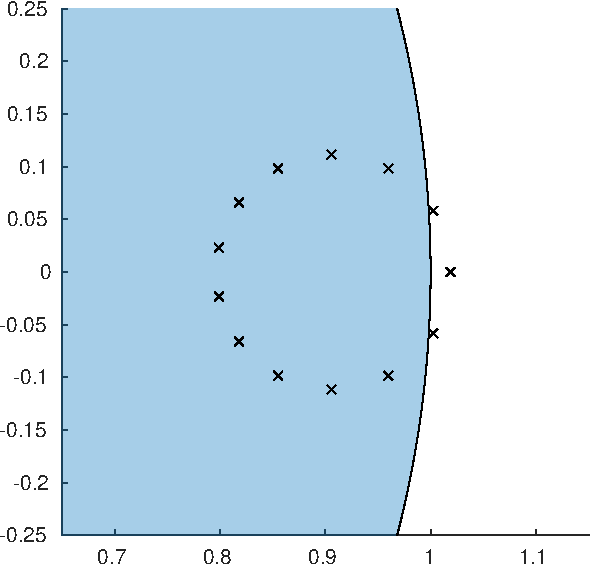
\includegraphics[height=0.35\textwidth]{qr13.pdf}
\caption{Disco unitario (in azzurro) e punti ottenuti\\
con il comando \texttt{roots(poly(0.9*ones(1,13)))}.}
\label{fig:qr13}
\end{figure}

Analizziamo ora un fenomeno interessante.
Se aumentassimo la molteplicità della radice 0.9 anche solo
di un'unità, il Programma \ref{prog:is-schur} inizierebbe a restituire esito
\code{false}, il che sappiamo essere sbagliato.
Potremmo dire semplicemente che l'algoritmo ha raggiunto
il suo limite di stabilità (il che non sarebbe poi sbagliato),
ma in verità c'è dell'altro.
Il fatto è che i coefficienti del polinomio $p(z)$
non possono essere rappresentati in modo esatto utilizzando i numeri
di macchina, quindi nel migliore dei casi saranno soggetti a una perturbazione
relativa dell'ordine dell'epsilon di macchina.
Per l'appunto, le radici del polinomio $p(z)$ sono estremamente sensibili
a una tale variazione, al punto da poter uscire dal disco unitario.
Nel Programma \ref{prog:schur-main} abbiamo calcolato la radice di modulo massimo
del polinomio $\tilde{p}(z)$ che si ottiene applicando la funzione
di arrotondamento $r(x)$ a ogni coefficiente del polinomio esatto $p(z)$
con esponente 14. È chiaro che questo è un caso favorevole:
meglio di così in precisione doppia non si può fare.
Il risultato del Programma \ref{prog:schur-main},
affidabile in quanto ottenuto con una precisione
di lavoro di 1000 cifre decimali, è circa 1.012:
il polinomio perturbato $\tilde{p}(z)$ non è quindi di Schur.
Allora, la colpa non è del Programma \ref{prog:is-schur},
tantomeno del comando \code{poly}:
è il problema stesso a essere mal condizionato,
al punto da rendere totalmente inadeguata la precisione
doppia offerta dai numeri a virgola mobile.

Alla luce di quest'ultime considerazioni, è chiaro che non avrebbe
senso scrivere in aritmetica inesatta la controparte del
Programma \ref{prog:is-schur} per polinomi di Von Neumann.
Tutti i polinomi di Von Neumann stabili rispetto a perturbazioni
dell'ordine dell'epsilon di macchina sono infatti anche polinomi di Schur.

\section{Modello del cobweb}

Il \emph{modello del cobweb} è un modello economico a tempo discreto
per la dinamica del prezzo di mercato $p$ di un bene soggetto a una
domanda $D$ e un'offerta $S$ esprimibili come funzioni
del solo prezzo $p$.
Affinché sia giustificata l'ipotesi di tempo discreto,
è necessario supporre che il bene non sia prodotto in modo continuativo,
bensì intermittente, cioè che sia soggetto a cicli di produzione.
Il modello del cobweb, pur essendo molto semplice, è in grado di riprodurre
sia dinamiche di mercato stabili, in cui il prezzo del bene tende a un valore
di equilibrio, sia dinamiche di mercato instabili, in cui il prezzo oscilla
in modo incontrollato.
Introduciamo in modo formale le grandezze economiche in gioco:
\begin{itemize}
\item $p_n$ è il prezzo a cui il bene viene scambiato sul mercato
	all'istante di tempo discreto $n$.
	In condizioni normali di mercato, il prezzo è una quantità positiva.
\item $D_n$ è la domanda del bene al tempo $n$.
	Supponiamo per semplicità che $D_n$ sia una funzione affine di $p_n$,
	cioè che esistano $a, d_0 \in \R$ tali che
	\[
	D_n = -a p_n + d_0.
	\]
	Secondo il principio per cui l'acquisto di un bene diminuisce
	all'aumentare del suo prezzo, il parametro $a$ ha segno positivo.%
	\footnote{Le rare eccezioni sono dette \emph{beni Veblen}.}
\item $S_n$ è l'offerta del bene al tempo $n$.
	L'ipotesi dei cicli di produzione già menzionata comporta
	che l'offerta al tempo $n$ debba essere pianificata al tempo $n-1$,
	in cui è noto lo storico dei prezzi $\{p_{n-1},\dots,p_0\}$,
	ma è ancora incognito il prezzo $p_n$ futuro.
	Supponiamo per il momento che il prezzo $p_n$ venga previsto tramite
	estrapolazione costante dei dati, cioè
	\[
	p_n = p_{n-1},
	\]
	e supponiamo anche che la strategia di produzione sia quella
	di adeguare l'offerta $S_n$ al prezzo previsto $p_n$ secondo
	una relazione affine. Allora esistono $b, s_0 \in \R$ tali che
	\[
	S_n = b p_{n-1} + s_0.
	\]
	Secondo il principio per cui la vendita di un bene aumenta
	al crescere del suo prezzo, il parametro $b$ ha segno positivo.
	È inoltre ragionevole supporre che l'offerta $s_0$ di un bene
	a prezzo nullo sia zero, o comunque enormemente inferiore alla domanda
	$d_0$ dello stesso bene a prezzo nullo.
\end{itemize}
%Supporre che le curve $D(p)$ e $S(p)$ siano polinomi di grado 1 non
%è ovviamente un'ipotesi molto realistica, tuttavia il modello
%del cobweb rimane
Per ottenere un sistema chiuso di equazioni, supponiamo infine che
il mercato operi in regime di concorrenza perfetta,
cioè che in ogni istante sia soddisfatta l'identità $D_n = S_n$.
Allora l'equazione alle differenze associata alla dinamica di $p_n$ è
\begin{equation} \label{eq:cobweb}
-a p_n + d_0 = b p_{n-1} + s_0
\qquad
a p_n + b p_{n-1} = d_0 - s_0.
\end{equation}
Osserviamo che una soluzione particolare di questa equazione
è data dalla soluzione costante
\[
p_n \equiv \frac{d0-s0}{a+b} \eqd \bar{p}.
\]
Il prezzo $\bar{p}$ è detto \emph{prezzo di equilibrio del bene},
ed è una quantità positiva grazie alle ipotesi sui parametri
del modello $d_0,s_0,a$ e $b$.
Il polinomio caratteristico dell'equazione omogenea associata alla
\eqref{eq:cobweb} è $az+b$, la cui unica radice è $-b/a$.
Allora, grazie alla formula \eqref{eq:soluzione-radici-multiple-non-omo},
possiamo scrivere la generica soluzione della \eqref{eq:cobweb}:
\[
p_n = \bar{p} + c_1 \left(-\frac{b}{a}\right)^n.
\]
Andando a imporre la condizione iniziale, otteniamo $c_1 = (p_0-\bar{p})$.

A questo punto è chiaro sotto quale condizione il prezzo sia stabile:
il parametro $a$ dev'essere maggiore di $b$, cioè,
a parità di incremento del prezzo, la variazione della domanda del bene
dev'essere maggiore della variazione dell'offerta.
In termini economici, si dice che la domanda dev'essere più \emph{elastica}
dell'offerta. Se $a > b$, allora il prezzo del bene tende al
prezzo di equilibrio $\bar{p}$ a partire da qualunque prezzo iniziale $p_0$.
Se $a = b$, il prezzo oscilla ma rimane limitato e positivo.
Infine, se $a < b$, il prezzo del bene oscilla in modo incontrollato
e si allontana dal prezzo di equilibrio; a un certo punto arriverà persino
ad assumere un valore negativo, segno che il mercato è entrato in crisi.

Vediamo ora due esempi numerici, uno relativo al caso stabile e uno al caso instabile:

\begin{esem}
Scegliamo come parametri del modello
\[
d_0 = 10, \quad
s_0 = 0, \quad
a = 1.5, \quad
b = 1, \quad
p_0 = 3.2, \quad
\texttt{nmax} = 10.
\]
Allora $a>b$ e quindi la dinamica è asintoticamente stabile: il prezzo $p_n$ tende a
\[
\bar{p} = (10-0)/(1.5+1) = 4.
\]
La successione dei prezzi è illustrata nella Figura \ref{fig:cobweb-stable}.
La tipica forma a ragnatela del grafico dà il nome al modello.
\end{esem}

\begin{figure}[bp]
\begin{subfigure}{0.45\textwidth}
	\centering
	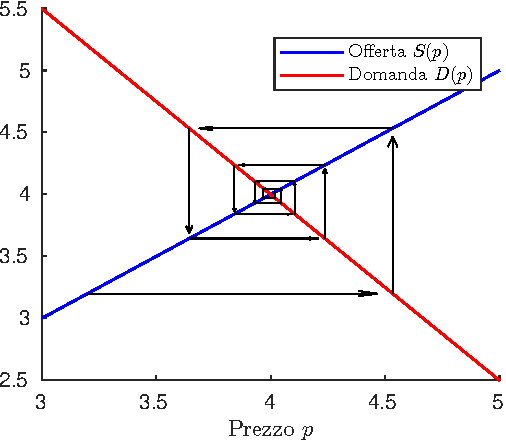
\includegraphics[width=\textwidth]{cobweb1.pdf}
	\caption{Dinamica stabile}
	\label{fig:cobweb-stable}
\end{subfigure}%
\hspace{0.04\textwidth}%
\begin{subfigure}{0.45\textwidth}
	\centering
	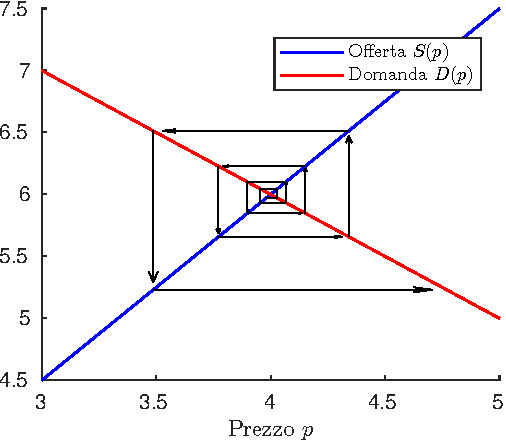
\includegraphics[width=\textwidth]{cobweb2.pdf}
	\caption{Dinamica instabile}
	\label{fig:cobweb-unstable}
\end{subfigure}
\caption{Simulazione numerica del modello del cobweb.}
\label{fig:cobweb}
\end{figure}

\begin{esem}
Scegliamo come parametri del modello
\[
d_0 = 10, \quad
s_0 = 0, \quad
a = 1, \quad
b = 1.5, \quad
p_0 = 3.98, \quad
\texttt{nmax} = 10.
\]
Allora $a<b$ e quindi la dinamica è instabile: nonostante il prezzo iniziale
sia molto vicino a quello di equilibrio, il prezzo $p_n$ diverge con un
andamento a spirale illustrato nella Figura \ref{fig:cobweb-unstable}.
\end{esem}

Il modello del cobweb può essere esteso andando a considerare
strategie di produzione più sofisticate. Per esempio, se il prezzo
$p_n$ venisse previsto tramite estrapolazione lineare, anziché
costante, si avrebbe $p_n = p_{n-1} + \rho(p_{n-1}-p_{n-2})$
per qualche $\rho \in \R$, e quindi
\[
S_n = b p_{n-1} + b \rho(p_{n-1}-p_{n-2}) + s_0.
\]
Il parametro $\rho$ del modello serve a regolare la quantità
di estrapolazione applicata.
Nel caso di cicli di produzione a intervalli di tempo regolari,
il valore $\rho = 1$ corrisponde a una strategia di estrapolazione lineare pura.
Valori di $\rho$ compresi tra $-1$ e $0$ corrispondono invece a scegliere
un prezzo intermedio tra $p_{n-1}$ e $p_{n-2}$
tramite una combinazione convessa.

L'equazione alle differenze associata alla dinamica di $p_n$ è
\[
a p_n + b (1+\rho) p_{n-1} - b \rho p_{n-2} = d_0-s_0,
\]
con polinomio caratteristico $az^2 + b (1+\rho) z - b \rho$.
Se $\rho \geq -1$, si può dimostrare che tale polinomio è di Schur se e solo se
\[
\frac{b}{a} < \frac{1}{\max\{\abs{\rho},1+2\rho\}}.
\]
Osserviamo che se il coefficiente di estrapolazione $\rho$ è positivo,
allora questa condizione è più stringente di quella vista
nel primo modello del cobweb ($a>b$),
mentre se il coefficiente è negativo allora è meno stringente.
Dunque, secondo le previsioni di questo semplice modello economico,
la strategia di pianificare la produzione di un bene cercando di anticipare
i prezzi futuri può portare a una destabilizzazione di mercati altrimenti stabili,
mentre la strategia di pianificare la produzione sulla base di una media dei prezzi
passati ha un effetto regolarizzante, che può portare all'equilibrio
mercati altrimenti instabili.

Concludiamo questo paragrafo con una simulazione del
modello del cobweb esteso tramite sostituzioni in avanti
(la Figura \ref{fig:cobweb} è stata generata utilizzando codice simile).
In questo caso i parametri del modello sono stati scelti in modo
che la dinamica risulti asintoticamente stabile e tenda al prezzo
di equilibrio $\bar{p} = 2$:

\vspace{1ex}
\lstinputlisting[frame=,label=prog:cobweb-esteso]{cobweb_esteso.m}
%caption={Simulazione numerica del modello del cobweb esteso.}

\section{Modello di economia di una nazione}

Analizziamo ora un altro modello economico a tempo discreto,
stavolta per la dinamica di un importante indicatore macroeconomico:
il prodotto interno lordo (PIL).
Il prodotto interno lordo $Y$ di una nazione può essere calcolato
su base annua come somma di quattro termini: i consumi finali delle famiglie $C$,
gli investimenti privati $I$, la spesa pubblica $G$ e la bilancia commerciale,
ossia il saldo tra esportazioni $X$ e importazioni $M$.
Questa approccio al calcolo del PIL è detto \emph{dal lato della spesa}.
Il fatto che il calcolo sia su base annua giustifica la scelta di
un modello a tempo discreto.
La dinamica del PIL è data dalle seguenti ipotesi semplificative:
\begin{itemize}
\item La bilancia commerciale è trascurabile, quindi
	\[
	Y_n = C_n + I_n + G_n.
	\]
\item I consumi finali delle famiglie al tempo $n$ sono una frazione
	del PIL al tempo $n-1$:
	\[
	C_n = \alpha Y_{n-1}, \quad \text{con $\alpha \in (0,1)$}.
	\]
\item Gli investimenti privati al tempo $n$ sono direttamente proporzionali
	alla crescita dei consumi:
	\[
	I_n = \rho(C_n-C_{n-1}), \quad \text{con $\rho > 0$}.
	\]
\item Le spese di governo sono costanti: $G_n \equiv G > 0$.
\end{itemize}
Tramite opportune sostituzioni, l'equazione $Y_n = C_n + I_n + G_n$
diventa quindi
\begin{equation} \label{eq:PIL}
Y_n = \alpha Y_{n-1} + \rho \alpha (Y_{n-1}-Y_{n-2}) + G,
\end{equation}
cioè un'equazione alle differenze che descrive l'evoluzione del PIL di anno in anno.
Come nel modello precedente, esiste un valore $\bar{Y}$ di equilibrio:
\[
\bar{Y} = \alpha \bar{Y} + \rho \alpha (\bar{Y}-\bar{Y}) + G
\qquad \bar{Y} = \frac{G}{1-\alpha} > 0.
\]
Tale valore sarà asintoticamente stabile se e solo se il polinomio
caratteristico $p(z)$ associato all'equazione \eqref{eq:PIL} è di Schur.
Si può dimostrare che
\[
p(z) = z^2 - \alpha(\rho+1)z + \alpha\rho,
\]
e che le sue radici sono nel disco unitario aperto se e solo se
$\alpha < 1$ e $\rho < 1/\alpha$.

Dunque, secondo le previsioni di questo semplice modello economico,
una strategia d'investimento troppo aggressiva,
specie se unita a consumi molto alti,
può avere un effetto destabilizzante sull'economia di una nazione.
Un esempio di dinamica instabile è riportato nella Figura \ref{fig:pil},
ottenuta con il Programma \ref{prog:pil} a partire da dati simili a quelli
del PIL italiano degli ultimi anni.
\vfill

\begin{figure}[hp]
\centering
\begin{tikzpicture}[trim axis left]
\begin{axis}[
	xlabel={$n$},
	ylabel={$Y_n$},
	xmin = 0, xmax = 19,
	ymin = 1000, ymax = 3000,
	width=0.5\textwidth,
	height=0.23\textheight
]
\addplot[blue] table {pil.dat};
\addplot[dashed, domain=0:19] expression {2000};
\end{axis}
\end{tikzpicture}
\caption{Dinamica instabile del prodotto interno lordo (in mld.\ di euro).}
\label{fig:pil}
\end{figure}

\lstinputlisting[float=hp,label=prog:pil,linerange={1-10},
caption={Simulazione numerica del modello di economia di una nazione.}]{pil.m}















